\chapter{Background}
\label{ch:background}

\textbf{Copied from IRP.}

This section aims to describe the most important components of this project. First, it provides a brief introduction to the RFID technology. It also explains the different types of RFID hardware. Then, the Raspberry Pi is discussed. Following subsections provide information about localisation principles and algorithms relevant to this project.

\subsection{Radio Frequency Identification (RFID)}

Radio frequency identification is a technology that has been used for remote identification since the 1950s \cite{Landt2005}. It has been developing since then. As it matures, it is becoming more inexpensive, which will likely create a vast range of opportunities for its application \cite{Nath2006}.

RFID can be considered an alternative and improvement of the current standard for identification of products, the barcodes.  Reading a barcode attached to an object requires a direct line of sight between a reader and a tag. In addition, barcodes can get obscured by other objects or substances, which hinders the identification process. RFID solves these disadvantages. It is a contactless technology that uses electromagnetic fields to carry information \cite{Finkenzeller2010}. Therefore, a direct line of sight is not required when reading data from tags attached to objects. RFID tags also support a larger set of unique IDs compared to bar codes, can be reprogrammed, and can store additional data depending on the application requirements. A RFID system has two compulsory hardware components, tags and readers.

A tag is a data-carrying device consisting of an antenna attached to a microchip both encapsulated in solid enclosure \cite{Finkenzeller2010}. Tags can be classified into two main categories, passive or active \cite{Want2006}. Passive tags do not require a power source. They communicate with readers by reflecting part of received radio waves, a term referred to as backscatter modulation \cite{Bolic2010}. Passive tags need to be in the readers' range to operate. Active tags require a power source in the form of a battery or are directly connected to the electrical grid \cite{Want2006}. Although, their lifetime might be limited by the available energy, active tags can be read from greater distances compared to passive tags.

A reader is a radio device that transmits radio waves and captures information send by tags. The reader's transmission frequency specifies the operational frequency of the RFID system, which is also their practical reading range \cite{Finkenzeller2010}. These devices usually consist of a radio frequency module, that capable of transmitting and receiving radio frequency signals, an antenna, and a control unit in the form of a microprocessor. 

\subsection{Raspberry Pi}

A single-board computer is a computer that is built on a single circuit board. It features most of the components of a personal computer. It has a processor, memory, storage, different microprocessors, and input/output interfaces. The Raspberry Pi is a particular implementation of a single-board computer. Figure \ref{fig:raspi} shows a graphical representation of its main components. Some of its strengths directly relating to this project are that it:
\begin{itemize}
 	\item has an affordable price that ranges from 25 to 35,
 	\item can be connected to a RFID reader through USB or GPIO pins,
 	\item is credit-card sized,
 	\item consumes little power (3.5 W).
\end{itemize}

\begin{figure}
	\begin{center}
		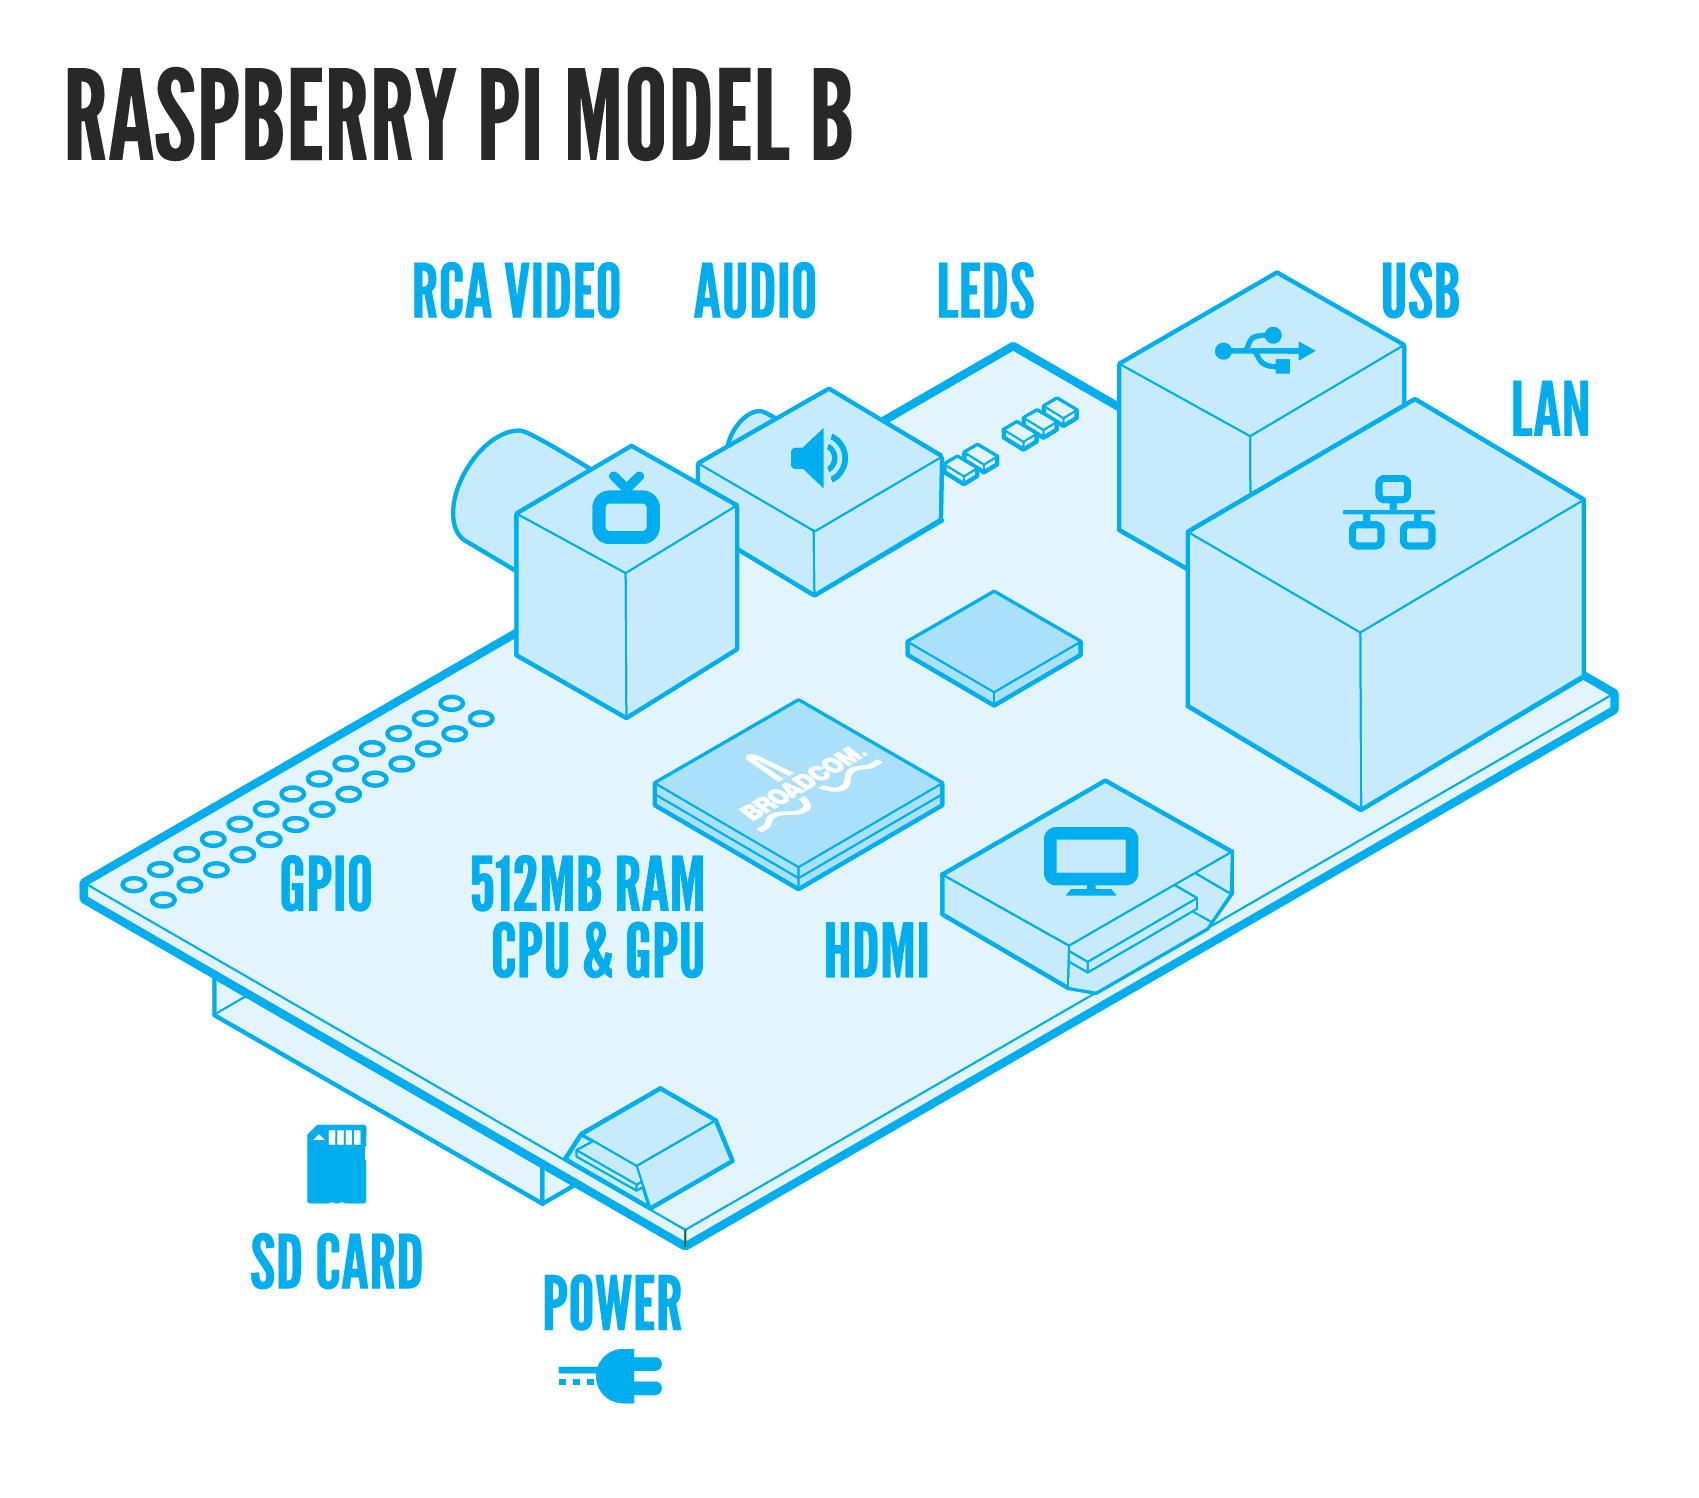
\includegraphics[width=0.6\textwidth]{figures/raspi}
		\label{fig:raspi}
		\caption{Raspberry Pi Model B. Figure from \url{http://www.raspberrypi.org/faqs}.}
	\end{center}
\end{figure}

\subsection{Distance estimation and localisation principles}

Some RFID readers can provide an indication of the strength of radio frequency signals received from tags. This metric is called Received Signal Strength Indicator (RSSI). Its value is usually output along with the identity information stored in a tag. It is estimated at the reader side before amplifying the received input. RSSI is a measurement of the power of the received strength represented as a value ranging from 0 to 255. It will be used in this project to estimate the distance between readers and a tag. This is done using a translation function that converts the RSSI values into a distance metric. Such a function will be developed for this project based the one used by the SpotON algorithm \cite{Hightower2000}.

Using the distances between readers and a tag, this project will employ the geometrical process of trilateration. It determines the relative position of a tag using properties of circles. The distance from a reader to a tag is the radius of a circle that could be drawn around the reader. The intersection of circles of three readers can be used to determine the approximate location of a tag relative to the readers. This technique has practical applications in surveying and navigation. Figure \ref{fig:lat} shows the concept of trilateration applied in the setting of this project.

\begin{figure}
	\begin{center}
		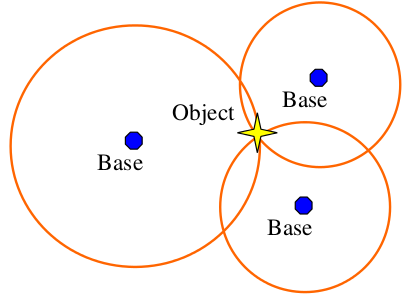
\includegraphics[width=0.45\textwidth]{figures/lateration}
		\label{fig:lat}
		\caption{The trilateration geometrical process applied in the context of this project. Figure from \cite{Hightower2000}.}
	\end{center}
\end{figure}

\section{Literature review}

\textbf{Copied from IRP.}

\subsection{SpotON}

SpotON is localisation algorithm based on lateration with distance estimation using RSS measurements. SpotON's operation involves a number of readers collecting signal strength information from active tags to determine their positions in the 3D space. At the time or their research, Hightower and his colleagues were using RFID hardware with 2-bit accuracy when measuring received signal strength \cite{Hightower2000}. They identified that this accuracy is not enough to achieve the precision required for localisation in small indoor environments. The authors mentioned that 8-bit accuracy (from 0 to 255) could be used in the future for improved results \cite{Hightower2000}. The SpotON algorithm consists of two main parts. First, RSS measurements are converted into a distance estimation. This is done using a translation function relying on numerical variables that were identified based on observation. This function is not generic and probably cannot be applied in this project. However, it will be analysed because it might provide important information about the relationships between RSS and distance. The next part of the algorithm is to apply a localisation algorithm that tries to minimise RSS errors \cite{Hightower2000}. It is based on the lateration geometrical process to estimate a position for an active RFID tag. This project will be using some of the methods and procedures applied in the SpotON system.

\textbf{Copied from project progress.}

It is a fine-grained tagging technology for 3D location sensing using radio signal strength analysis. They tried to develop a low cost system compared to commercial solutions available at their time. They believe that the accuracy and efficiency of location sensing could be enhanced by sensor fusion, i.e. adding more sensors (accelerometers) and building maps. These authors talk about ubiquitous computing. They try to separate the meanings of positioning and tracking. Positioning is concerned with providing means to calculate location which can be used to compute an actual position. Tracking is monitoring objects without involving them in the computation. They define location sensing to be such systems that separate the manipulation of location data from the mechanisms of actually pinpointing the objects. They used radio devices with a serial connection similar to the devices that will be used in this project. They were talking about the limitations of such a serial connection (R232) which will mitigated in our case by using a converter from serial to USB. In our case base stations that aggregate information and a server that processes it is combined into the Raspberry Pi computer. 
	
This paper summarises the localisation algorithm they used based on the conversion of distance into signal strength in 6 directions in 3D. Then the measured RSS is compared to the 6 known RSS to find a location around a reader. They do not store data or timing information on the server, which I am planning to do. They have a visualisation client written in OpenGL. 
	
Their results are not very accurate because they use radio devices with 2-bit RSS accuracy compared to modern onces with 8-bit accuracy. Their second problem was measurement frequency which happened between 10 to 20 seconds, which is too slow to monitor real-time position changes of objects. They identified these limitations and solved them by creating a custom hardware.

\subsection{An Introduction to RFID Technology \cite{Want2006}}

\textbf{Copied from project progress.}

Read and highlighted "An Introduction to RFID Technology" by Roy Want \cite{Want2006}. It is good introductory article that clearly explains different classifications of RFID. It has helpful graphics for the distinction between near and far field RFID communication.

\subsection{RFID Tags: Positioning Principles and Localization Techniques \cite{Bouet2008}}

Contains similar introduction to RFID technology. Explains the role of the server (RasPi in our case) connected to the readers that runs a localisation algorithm and provides the middleware for communication between servers. Contains a good classification of indoor localisation algorithms - distance estimation, scene analysis, and proximity. A brief but clear explanation of lateration with a useful figure. Contains a classification of range measurements techniques starting with Received Signal Strength (RSS) that will be used in this project. "The attenuation (gradual loss) of emitted signal strength is a function of the distance between the emitter and the receiver."

A classification of different RFID localisation schemes is proposed. The first one is SpotON where multiple readers collect RSS measurements in order to approximate distance from the tag. Then lateration is performed to localise the tag. 
	
Landmarc is another approach that uses reference tags that are regularly deployed on the covered area. The idea here is to select the k nearest reference tags that are closest to the unknown tag using differences in RSS measurements. Having identified the k nearest reference tags their coordinates are used to localise the unknown tag. 
	
VIRE extends the methods used in Landmarc by defining a proximity map that every reader records. This proximity map consists of a 2D grid of reference tags where the centre of a cell is a tag. The difference in the RSS measurements between reference and unknown tag helps label cells in the proximity map so that it can be constructed. The union of individual proximity maps gives a global proximity map for the unknown tag.
	
Simplex is a method that requires different transmission power levels. I am not sure if our equipment has this feature.
	
A Kalman filtering method is briefly explained but have to read the original paper because it is hard to understand from a one paragraph description of the method.
	
Scout is a probabilistic localisation technique that uses a probabilistic RSS model to estimate distances from a tag to readers. Predicted beliefs are calculated and corrected using reference tags until a good model is constructed.

\subsection{Semantic Sensor Net: An Extensible Framework\cite{Ni2005}}

It is more concerned with sensor networks with multiple nodes, where the nodes have less importance than traditional computer networks. The article proposes an extensible framework for sensor networks that relies on attaching semantics (meanings) to sensor data but also to sensor nodes, location, context, and queries. The idea is to attach a meaning to every piece of information so that those meanings can be used by the network to route and aggregate data more efficiently, for example. This paper does not have a direct connection to this project but gives grounds for thoughts about attaching meaning to measurements, considering heterogeneous RFID reader nodes, and taking scalability into account.

\subsection{LANDMARC: Indoor Location Sensing Using Active RFID \cite{Ni2004}}

LANDMARC is a location sensing system that uses RFID for locating objects inside buildings. Its major advantage is that it improves the overall accuracy of locating objects by using reference tags. They believe that the choice of technology and techniques is of crucial importance for the granularity and accuracy of the location information. They identify that range of a RFID system is determined by the power available at readers and tags and the environmental conditions and structures. In free space, the signal strength reduces in inverse proportion to the square of the distance. They found out that instead of using a lot of readers, they can arrange a number of tags in a 2D rectangular grid to use as reference tags. They associate reference tags with landmarks that help navigation in a city, for example. The advantage is that tags are cheaper and are subject to the same environmental factors as the tags being tracked. The authors believe that the placement of readers and reference tags is very important for the accuracy of the system. They needed an algorithm to connect the relationships between signal strengths and power levels that the readers return.
	
Their setup consists of RF tags and readers with a wireless module for communicating measurements to a location server. Their methodology is explained very good in their paper and relies on Euclidean distance between reference tags and unknown tags and also on k nearest neighbours to pinpoint a possible position. They apply a weighing factor when computing coordinates. To measure the accuracy of the system error distance is used. It is the linear distance between real coordinates and computed coordinates.
	
They discuss different parameters of the system. First, they found through experimentation that 4 nearest neighbours provide the best results during most of their tests. They also acknowledge the environmental factors night vs. day tests, change of placement of the tracking tags. They have restricted the number of readers used but point out that more readers provide better accuracy in certain cases. The LANDMARC system is based on reference tags so the authors discuss in detail the placement and number of the reference tags. They argue that density of reference tags plays an important role for the accuracy of the system. A good setup, they used, was consisting of 4 readers and 1 reference tag per square meter resulting in an average distance error of 1 meter.
	
Back in 2004 when the paper was written, the authors identified the hardware problems of the current RFID technology. None of RFID products supplied signal strength directly which requires unnecessary processing and sacrifice of accuracy. They also were complaining about the long latency between actual placement of tracking tags and the system computing their location. Two factors were contributing to this problem. One being the scanning time of the readers, not supporting RSS. The second the time interval of a tag emitting its ID, which is not a configurable parameter. They also identified different power levels detected by a reader from two tags which resulted in variation in their behaviour.

\subsection{Location Estimation Technique using Extended 3-D LANDMARC Algorithm for Passive RFID Tag \cite{Khan2009}}

It is an extension of LANDMARC for 3D. They used passive instead of active tags. They use RSSI which is availble from the readers they used instead of computing it from power levels. The error rate they recorded was 0.5m when estimating location. The authors explain what RSS is and summarise relationships between RSS values and distance metrics for outdoor and indoor environments. They explain that RSS measurements may suffer from multi-path fading, shadowing, diffraction, reflection, and scattering. They explain what scene analysis (finger printing) is and the two phases it consists of (offline and online). They summarise the main methods used with scene analysis: probabilistic, kNN, and neural networks. They use the same methodology as the original LANDMARC system but extend it to 3D, adding 'z' coordinate. For their experiments they used 3 readers, 2 tracking tags, and 11 reference tags. They supply all their intermediate and final results in tables with computed values for RSS tag vectors, Euclidean distance between reference and tracking tags, weights for every distance, reference tags coordinates, and estimated tracking tag's coordinates.



\section{Summary}
